\addcontentsline{toc}{chapter}{ภาคผนวก A}
\chapter{โปรแกรมที่พัฒนาขึ้น}
\section{โปรแกรมทดสอบ}
\hspace{1cm} สำหรับโครงงานวิจัยเรื่องนี้เป็นการพัฒนาวิธีเชิงตัวเลข การจะวัดประสิทธิภาพของวิธีการเชิงตัวเลขได้ จำเป็นจะต้องใช้โปรแกรมเข้าทดสอบ โดยโครงงานวิจัยนี้ มีโปรแกรมสำหรับทดสอบ ซึ่งสามารถแบ่งได้ออกเป็น 2 ส่วนคือโปรแกรมสำหรับทดสอบขั้นตอนการซ่อมแซมภาพศิลปะไทยและการลบคำบรรยายอนิเมะ
\subsection{โปรแกรมทดสอบการซ่อมแซมภาพศิลปะไทย}
\hspace{1cm} โดยโค้ดของโปรแกรมสามารถดาวน์โหลดได้ที่ https://github.com/pureexe/YaeProgression01-color-image เป็นโค้ดภาษา C++ โดยถูกพัฒนาบน Visual Studio 2017 และจำเป็นต้องคอมไพล์โค้ดก่อนใช้งาน ทั้งนี้ท่านสามารถดาวน์โหลดไฟล์ที่่คอมไพล์เรียบร้อยสำหรับ Windows 64 bit ได้ที่ https://github.com/pureexe/YaeProgression01-color-image/releases

\hspace{1cm} โดยการรัน ให้เปิด command prompt โดยการ เปิดปุ่ม Windows+R จากนั้นพิมพ์ cd "ชื่อโฟลเดอร์" ที่ได้ทำการดาวน์โหลด releases มาแตกไฟล์ไว้ จากนั้นใช้คำสั่ง cd "application" เพื่อเข้าไปโฟลเดอร์ที่มีไฟล์โปรแกรมอยู่ แล้วจึงใช้คำสั่ง labarotory.exe เพื่อทำการทดสอบ โดยไฟล์ผลลัพธ์จากการทดสอบจะปรากฏในโฟลเดอร์ result และจะแสดงเวลาที่ใช้ในการประมวลผลออกทางหน้าจอ

\begin{figure}[H]
    \centering
    \begin{subfigure}{0.8\linewidth}
        \centering
        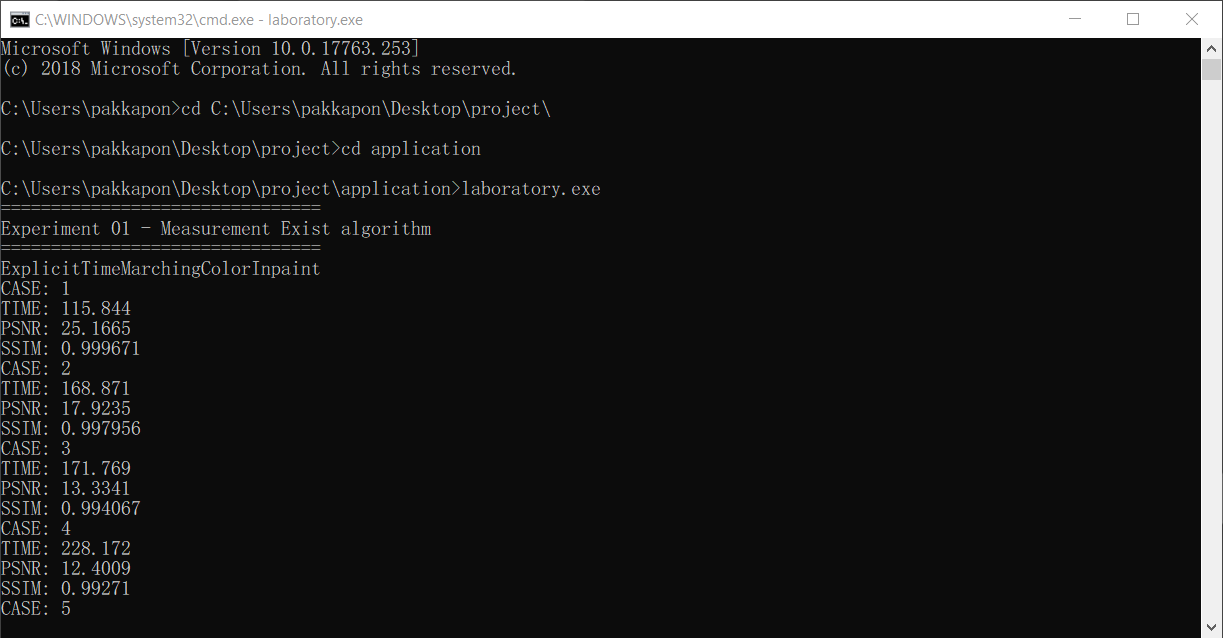
\includegraphics[width=1\linewidth]{image/software_appendix/laboratory.png}
    \end{subfigure}
    \caption{ตัวอย่างโปรแกรมสำหรับทดสอบการซ่อมแซมภาพศิลปะไทยที่พัฒนาขึ้น}
\end{figure}

\subsection{โปรแกรมทดสอบการลบบทบรรยายจากอนิเมะ}
\hspace{1cm} สำหรับโปรแกรมทดสอบการลบคำบรรยายอนิเมะนั้น เขียนด้วยภาษา power shell เพื่อใช้ในการทดสอบ โดยเครื่องที่จะนำไปทดสอบ จำเป็นต้องติดตั้ง ffmpeg, MPC-HC, Avisynth+ และ OpenCV ซึ่งเมื่อติดตังแล้วสามารถทำการทดสอบได้โดยการเรียกใช้สคริปนี้ https://github.com/pureexe/matlab-inpaint-speed-analysis/blob/master/experiment-08/taskrunner/test-algorithm/test-20181111.ps1

\begin{figure}[H]
    \centering
    \begin{subfigure}{0.8\linewidth}
        \centering
        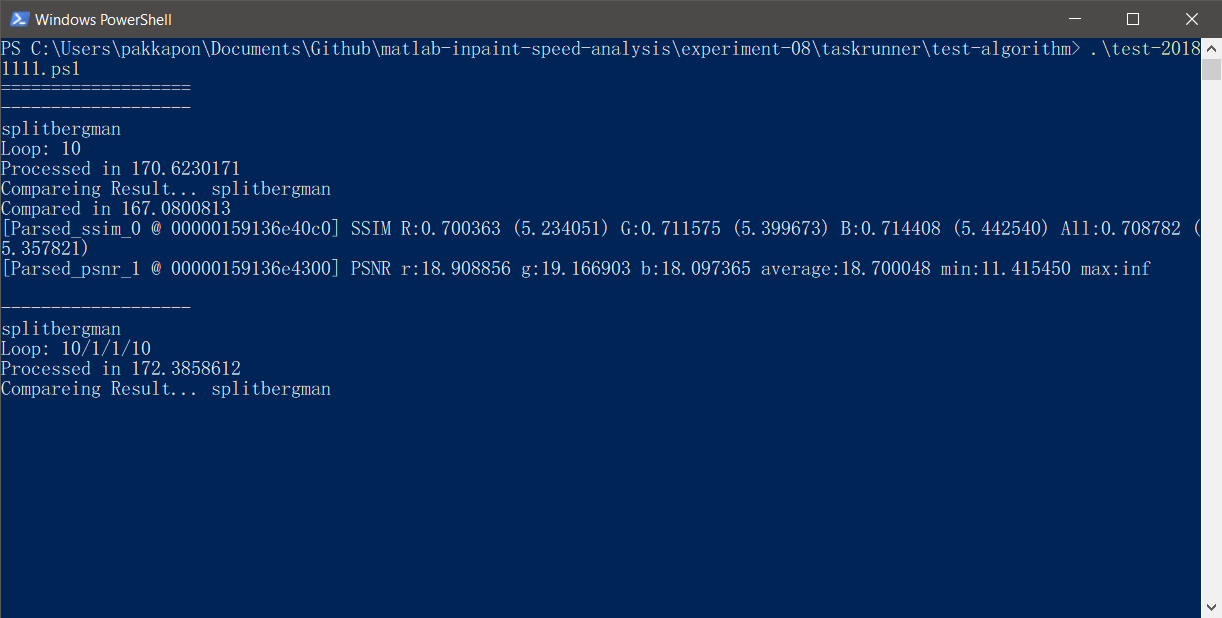
\includegraphics[width=1\linewidth]{image/software_appendix/lab_remove.png}
    \end{subfigure}
    \caption{ตัวอย่างโปรแกรมสำหรับทดสอบการลบคำบรรยายที่พัฒนาขึ้น}
\end{figure}

\hspace{1cm} นอกจากนี้ในส่วนของการตรวจว่าขั้นตอนการหาคำบรรยายนั้นสามารถทำได้ดีเพียงใด สามารถทดสอบได้โดยการรันสคริปนี้ https://github.com/pureexe/matlab-inpaint-speed-analysis/blob/master/experiment-09/taskrunner/compare-mask/test-20181112.ps1

\begin{figure}[H]
    \centering
    \begin{subfigure}{0.8\linewidth}
        \centering
        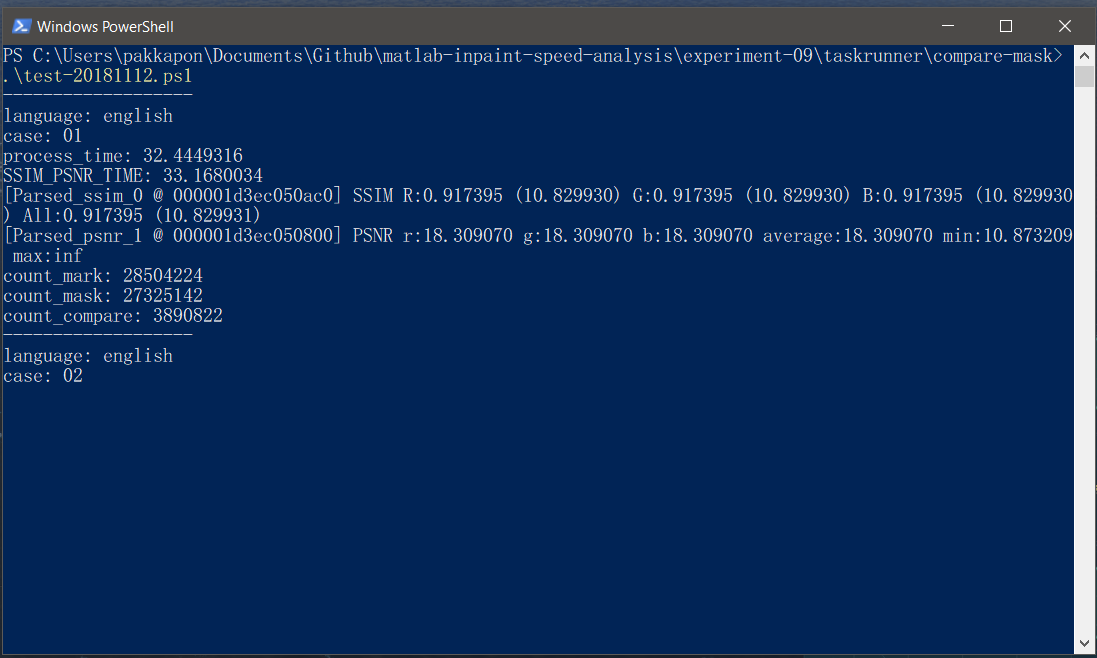
\includegraphics[width=1\linewidth]{image/software_appendix/lab_find.png}
    \end{subfigure}
    \caption{ตัวอย่างโปรแกรมสำหรับทดสอบการหาคำบรรยายที่พัฒนาขึ้น}
\end{figure}


\section{โปรแกรมตัวอย่างการซ่อมแซมภาพศิลปะไทย}
\hspace{1cm} เนื่องจากโปรแกรมสำหรับทดสอบที่ได้สร้างขึ้นมานั้นมีข้อจำกัดด้านอุปกรณ์ ซึ่งรองรับเพียง Windows 64 bit เท่านั้น ทำให้ไม่สามารถทำงานได้บนอุปกรณ์อื่นๆ ทางผู้วิจัยจึงได้ทำการเขียนที่พัฒนาขึ้นใหม่ให้ใช้งาน บน Google Colab ได้ ซึ่งสามารถเข้าใช้งานได้ที่ https://bit.ly/thai-inpaint-colab ซึ่งนอกจากตัวอย่างที่เตรียมไว้ให้จำนวน 5 ภาพแล้ว ยังสามารถอัปโหลดภาพที่เสียหายพร้อมทั้งโดเมนสำหรับการต่อเติมเพื่อทำการซ่อมแซมภาพได้อีกด้วย

\begin{figure}[H]
    \centering
    \begin{subfigure}{0.8\linewidth}
        \centering
        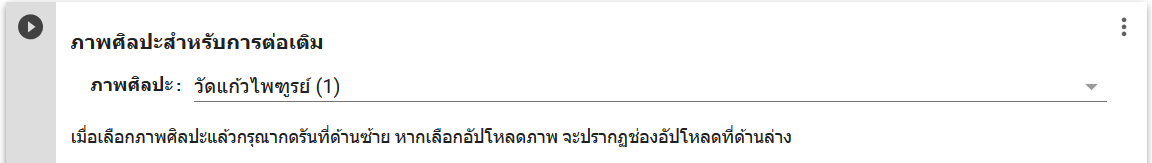
\includegraphics[width=1\linewidth]{image/appendix_colab/select_image.png}
    \end{subfigure}
    \caption{ตัวอย่างการเลือกรูปภาพสำหรับทำการทดสอบ}
\end{figure}
\begin{figure}[H]
    \centering
    \begin{subfigure}{0.8\linewidth}
        \centering
        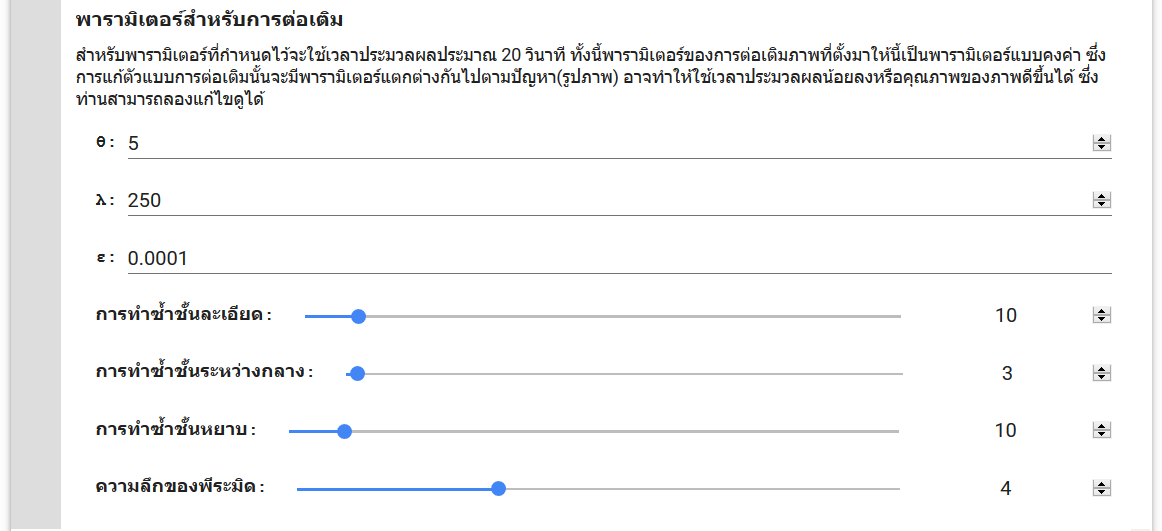
\includegraphics[width=1\linewidth]{image/appendix_colab/select_parameter.png}
    \end{subfigure}
    \caption{ตัวอย่างการปรับค่าพารามิเตอร์ที่ใช้ในโครงงานวิจัยนี้}
\end{figure}
\begin{figure}[H]
    \centering
    \begin{subfigure}{0.8\linewidth}
        \centering
        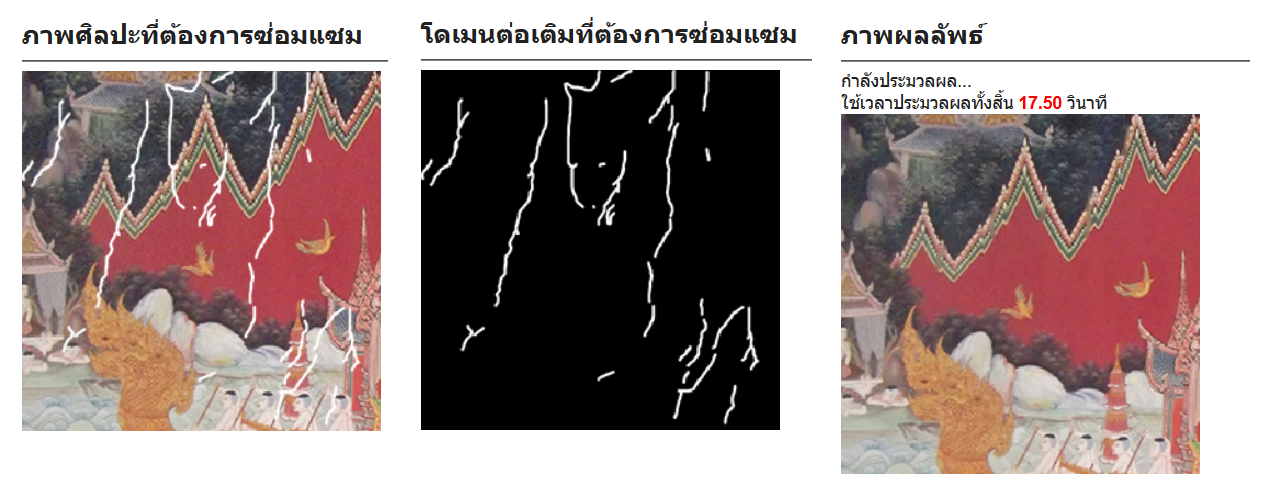
\includegraphics[width=1\linewidth]{image/appendix_colab/inpaint_display.png}
    \end{subfigure}
    \caption{ตัวอย่างภาพผลลัพธ์จาก Google Colab}
\end{figure}

\section{โปรแกรมตัวอย่างการลบบทบรรยายจากอนิเมะ}
\hspace{1cm} สำหรับการลบคำบรรยายอนิเมะนั้น ขณะนี้ยังรองรับเพียงขอบบทบรรยายที่เป็นสีดำเท่านั้น เครื่องคอมพิวเตอร์ที่จะใช้งาน จะต้องเป็น Windows 64 bit ที่มีการติดตั้ง MPC-HC, Avisynth+ และ OpenCV เสียก่อน จากนั้นดาวน์โหลดตัวอย่างได้ที่ http://bit.ly/demo-anime-inpaint เมื่อทำการแตกไฟล์ให้เปิดไฟล์ SubtitleRemove.avs ด้วย MPC-HC เพื่อแสดงตัวอย่าง และสามารถนำไฟล์ตัวอย่างนี้ไปใช้กับวิดีโออนิเมะอื่นได้โดยทำการเปิด SubtitleRemove.avs ด้วยโปรแกรม Text Editor อื่นๆ เช่น Notepad++ เพื่อแก้ไขพารามิเตอร์ Top, Bottom, Left และ Right เพื่อระบุที่อยู่ตำแหน่งของคำบรรยายในหน่วยพิกเซล อีกทั้งแก้ไขพารามิเตอร์ StokeWidth เพื่อแก้ไขตัวความหนาของคำบรรยายในหน่วยพิกเซล

\begin{figure}[H]
    \centering
    \begin{subfigure}{0.8\linewidth}
        \centering
        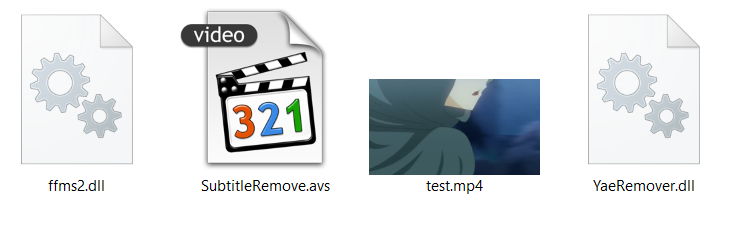
\includegraphics[width=1\linewidth]{image/demo_anime/file.png}
    \end{subfigure}
    \caption{ไฟล์ตัวอย่างเมื่อทำการแตกไฟล์ออกมาแล้ว test.mp4 เป็นวิดีโอมีมีคำบรรยาย และ SubtitleRemove.avs เป็นโปรแกรมตัวอย่างสำหรับลบคำบรรยาย}
\end{figure}
\begin{figure}[H]
    \centering
    \begin{subfigure}{0.8\linewidth}
        \centering
        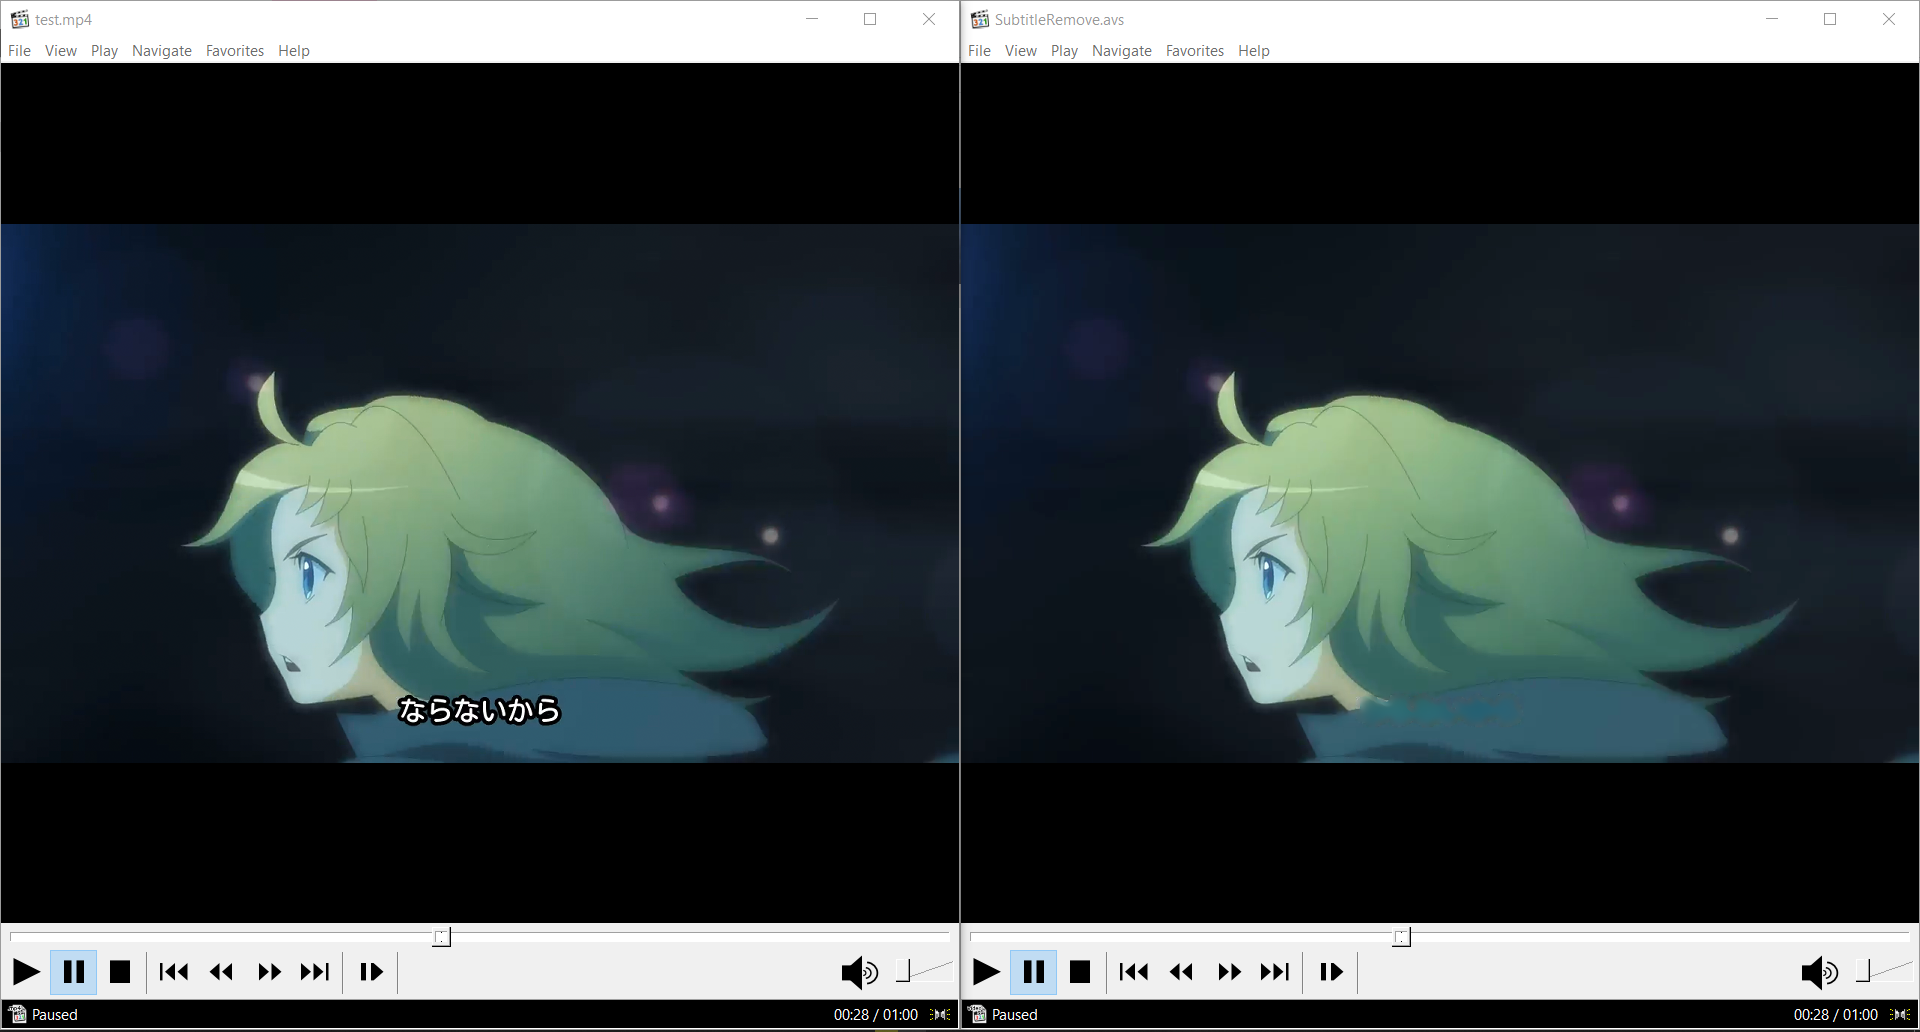
\includegraphics[width=1\linewidth]{image/demo_anime/result.png}
    \end{subfigure}
    \caption{(ซ้าย) test.mp4 (ขวา) SubtitleRemove.avs เมื่อเปิดด้วย MPC-HC}
\end{figure}
\begin{figure}[H]
    \centering
    \begin{subfigure}{0.8\linewidth}
        \centering
        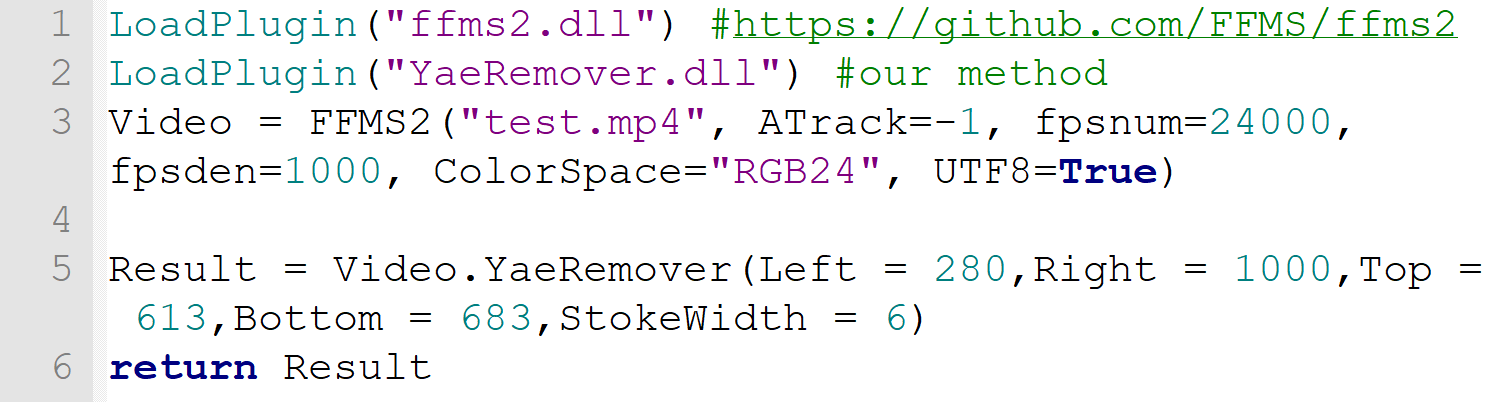
\includegraphics[width=1\linewidth]{image/demo_anime/notepad.png}
    \end{subfigure}
    \caption{SubtitleRemove.avs สามารถแก้พารามิเตอร์เพื่อใช้กันวิดีโออนิเมะอื่นได้}
\end{figure}